\chapter{Usar GitHub como repositorio remoto}
\href{https://github.com/}{GitHub} es un portal donde podemos crear repositorios para poder usarlo como sistema centralizado de nuestros proyectos.

Entre las característica que tiene, se pueden destacar:
\begin{itemize}
    \item Entorno gráfico para controlar el repositorio. Se puede ver el histórico del repositorio, quién ha realizado los cambios, cuándo, ramas creadas...
    \item Control de incidencias. Para poder crear “\textit{issues}” del proyecto a medida que encontremos errores.
    \item Generar documentación por proyecto en formato Wiki.
    \item Gestión de “\textit{pull requests}” para integrar cambios en la rama principal.
    \item Sistema de “acciones”, que ayudan para el sistema de “integración continua”. Con estas acciones podemos generar “\textit{releases}”, compilar el código y comprobar si hay errores, pasar tests, ... Hay mucha \href{https://docs.github.com/en/actions}{documentación} al respecto.
\end{itemize}

\section{Crear repositorio}

Una vez hemos creado una cuenta, podremos crear un nuevo repositorio en la plataforma. Al crearlo, podemos elegir distintas configuraciones:

\begin{itemize}
    \item \textbf{Nombre del repositorio}, para poder acceder a él. Es recomendable darle un nombre significativo al proyecto.
    \item \textbf{Descripción}, donde podremos indicar un poco de texto para entender de qué trata el proyecto.
    \item \textbf{Visibilidad}. Podemos hacer que el repositorio sea \textbf{público} (cualquier persona puede ver el contenido del proyecto) o \textbf{privado} (sólo nuestro usuario puede verlo).

    \item \textbf{Inicializar el proyecto con}: Podemos hacer que cuando Github inicialice el proyecto le añada ciertos ficheros:
    \begin{itemize}
        \item \textbf{README}: Fichero donde indicar de qué trata el fichero, cómo compilarlo, ...
        \item \textbf{.gitignore}: Un fichero que nos permite ignorar ficheros dentro de nuestro “área de trabajo”. Podemos elegir de una plantilla para distintos lenguajes de programación.
        \item \textbf{Licencia}: Un fichero con distintas licencias libres para nuestro proyecto.
    \end{itemize}
\end{itemize}


\begin{center}
    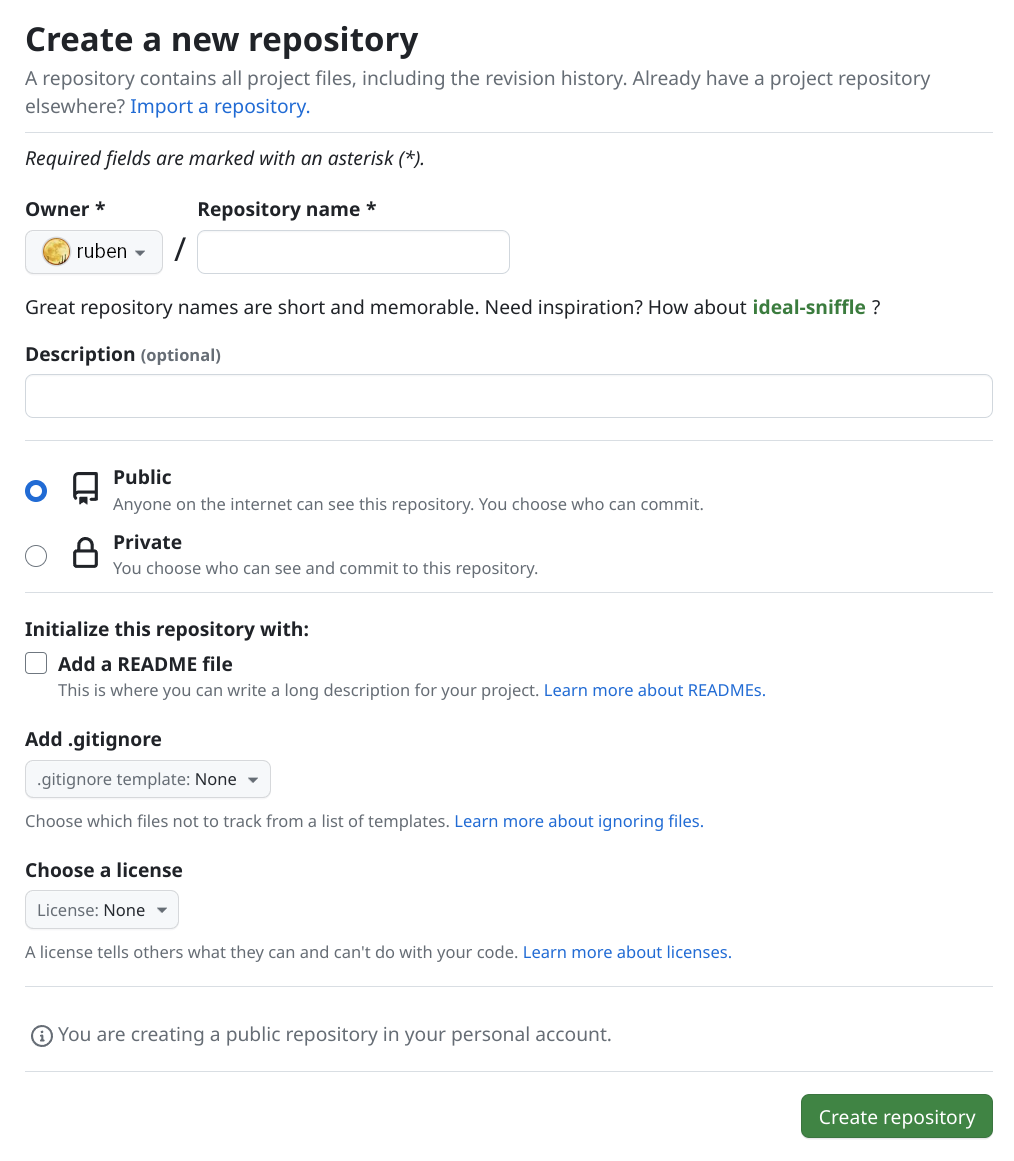
\includegraphics[frame,width=0.7\linewidth]{github-new.png}
    \captionof{figure}{Opciones al crear un nuevo repositorio en GitHub}
\end{center}

En este caso se va a crear un repositorio público llamado \textbf{pruebas}, sin ningún tipo de fichero. De esta manera “enlazaremos” el repositorio local de los pasos anteriores con este repositorio.


\chapter{Enlazar repositorio con remoto}

GitHub nos muestra cuáles son los pasos para enlazar un repositorio existente con el que acabamos de crear en su plataforma, a través de la línea de comandos:

\begin{mycode}{Enlazando repositorio local con uno en GitHub}{console}{{\small }}
ruben@vega:~/pruebas$ git remote add origin git@github.com:yuki/pruebas.git
ruben@vega:~/pruebas$ git branch -M main
ruben@vega:~/pruebas$ git push -u origin main
\end{mycode}

Vamos a tratar de entender qué es lo que hace cada uno de los comandos, ya que es importante.

\begin{itemize}
    \item \commandbox{git remote add origin git@github.com:yuki/pruebas.git}

    Con este comando se añade un repositorio remoto con el nombre “\textbf{origin}”. Básicamente estamos diciéndole al repositorio local que cuando realicemos algo sobre el repositorio remoto “origin” haga uso de esa URL.

    El nombre “origin” se puede cambiar, pero es el nombre que decidieron ponerle:

    \begin{center}
        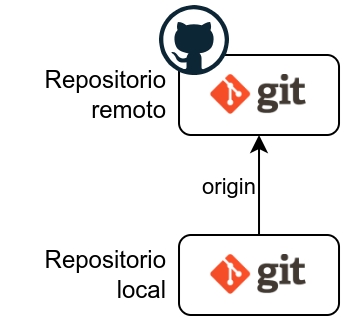
\includegraphics[width=0.7\linewidth]{remote.png}
        \captionof{figure}{Enlazamos repositorio local con remoto de nombre “origin”}
    \end{center}

    \item \commandbox{git branch -M main}

    Este comando lo que hace es cambiar el nombre de la rama principal para que se llame “\textbf{main}”. Originalmente la rama principal se llamaba “master”, pero en 2020 decidieron cambiarlo a “main”.

    En las nuevas versiones de git “main” ya es el nombre por defecto, por lo que este comando puede no ser necesario (si se ejecuta no hace nada).

    \item \commandbox{git push -u origin main}

    Este comando se puede separar en dos partes:
    \begin{itemize}
        \item \commandbox{git push}

        Este es el comando que utilizaremos para enviar al repositorio remoto los commits que hemos realizado en el repositorio local.

        \item \commandbox{-u origin main}

        Estos parámetros sólo los usaremos para realizar el primer envío. Estos indican al repositorio local que haga uso del servidor remoto “origin” para enlazar la rama en la que nos encontramos (“main”) con la rama remota “main” a la hora de enviar las revisiones.

        Los nombres de las ramas no tienen por qué coincidir, pero que sean iguales nos va a facilitar identificar ambas.

        \begin{center}
            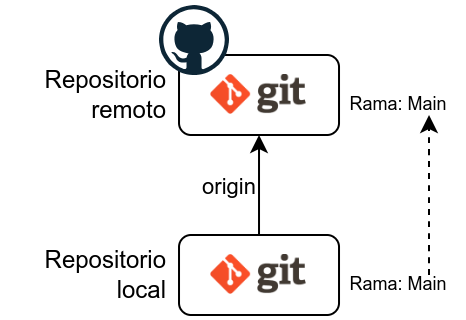
\includegraphics[width=0.7\linewidth]{remote_push.png}
            \captionof{figure}{Enlazamos rama local con rama remota}
        \end{center}
    \end{itemize}

\end{itemize}

Al realizar el último comando en windows nos aparecerá una ventana para que realicemos el \textbf{login de usuario} en GitHub.

\section{Añadiendo credenciales de acceso en Windows}

Dado que realizar una modificación en un repositorio de GitHub es algo que puede puede conllevar un peligro en el código fuente, nos aparecerá una ventana para que realicemos el login de usuario.

\begin{center}
    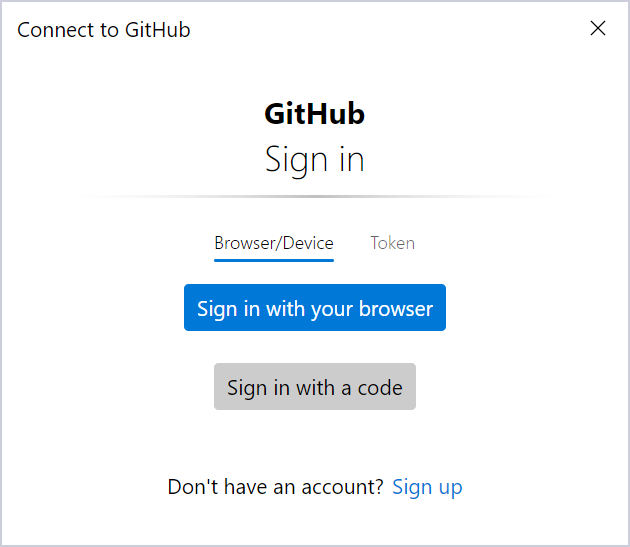
\includegraphics[frame,width=0.5\linewidth]{github_login.png}
    \captionof{figure}{Ventana para realizar el login en GitHub}
\end{center}

Elegiremos la opción marcada en azul, lo que nos abrirá el navegador web para realizar el login en la web de GitHub. Una vez hayamos introducido bien los credenciales de acceso, veremos la confirmación. Esto nos creará una autenticación “OAuth de aplicación” en \href{https://github.com/settings/applications}{nuestro perfil de GitHub} (Usuario → Settings → \href{https://github.com/settings/applications}{Applications}), pestaña “\textit{Authorized OAuth Apps}”.

\begin{center}
    
\includegraphics[frame,width=0.5\linewidth]{github_login2.png}
    \captionof{figure}{Login realizado correctamente}
\end{center}

Y para que siga funcionando, en el \textbf{Administrador de Credenciales} de Windows (“Panel de Control → Cuentas de Usuario → Administrador de Credenciales → Credenciales de Windows”), también nos creará una entrada nueva de credenciales genéricas:

\begin{center}
    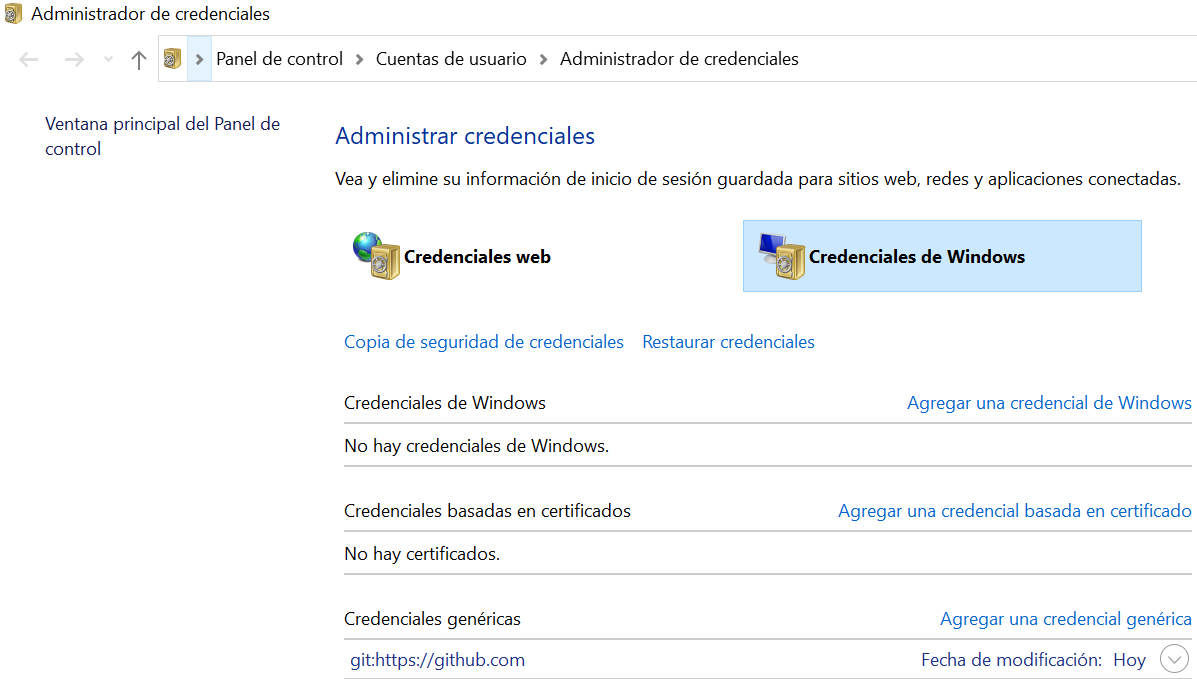
\includegraphics[frame,width=0.9\linewidth]{windows_credentials.png}
    \captionof{figure}{Credenciales de GitHub en Windows}
\end{center}

Una vez realizados estos pasos, nos funcionará el comando y enlazará la rama y enviará los commits realizados al servidor remoto.

\begin{mycode}{Enlazando la rama y enviando los cambios}{console}{}
ruben@vega:~/pruebas$ git push -u origin main
Enumerando objetos: 10, listo.
Contando objetos: 100% (10/10), listo.
Compresión delta usando hasta 6 hilos
Comprimiendo objetos: 100% (7/7), listo.
Escribiendo objetos: 100% (10/10), 889 bytes | 222.00 KiB/s, listo.
Total 10 (delta 2), reusados 0 (delta 0), pack-reusados 0
remote: Resolving deltas: 100% (2/2), done.
To github.com:yuki/pruebas.git
* [new branch]      main -> main
rama 'main' configurada para rastrear 'origin/main'.
\end{mycode}


\chapter{Enviar modificaciones locales}

A partir de ahora, cualquier modificación que hayamos realizado en local \textbf{deberemos enviarla al servidor remoto}. No tenemos por qué hacerlo por cada commit, ya que cuando realicemos el envío se enviarán todos los que no estén en remoto.

\begin{mycode}{Enlazando la rama y enviando los cambios}{console}{}
ruben@vega:~/pruebas$ git push
git push
Enumerando objetos: 5, listo.
Contando objetos: 100% (5/5), listo.
Compresión delta usando hasta 6 hilos
Comprimiendo objetos: 100% (3/3), listo.
Escribiendo objetos: 100% (3/3), 324 bytes | 324.00 KiB/s, listo.
Total 3 (delta 1), reusados 0 (delta 0), pack-reusados 0
remote: Resolving deltas: 100% (1/1), completed with 1 local object.
To github.com:yuki/pruebas.git
cefb314..2cac944  main -> main
\end{mycode}


\chapter{Clonar repositorio remoto}

Imaginemos que una vez subido los cambios locales a GitHub queremos hacer uso del repositorio en otro ordenador. Para ello, debemos realizar un “clonado” del repositorio en cuestión.

\begin{mycode}{Clonar repositorio remoto en repositorio local}{console}{}
ruben@vega:~/pruebas$ git clone https://github.com/yuki/pruebas.git
Clonando en 'pruebas'...
remote: Enumerating objects: 20, done.
remote: Counting objects: 100% (20/20), done.
remote: Compressing objects: 100% (12/12), done.
remote: Total 20 (delta 4), reused 20 (delta 4), pack-reused 0
Recibiendo objetos: 100% (20/20), listo.
Resolviendo deltas: 100% (4/4), listo.
\end{mycode}


\chapter{Obtener últimos commits}

Si alguien ha realizado commits en nuestro repositorio (o los hemos realizado nosotros desde otro ordenador), es posible que nuestro repositorio local no esté actualizado. Para actualizarlo tenemos que entender dos comandos:

\begin{itemize}
    \item \commandbox{git fetch}

    Obtiene los commits del repositorio remoto, \textbf{pero no los aplica sobre nuestra copia de trabajo actual}. De esta manera, no se aplican los cambios y mientras tanto podemos seguir trabajando.

\begin{mycode}{Titulo}{console}{}
ruben@vega:~/pruebas$ git fetch
remote: Enumerating objects: 5, done.
remote: Counting objects: 100% (5/5), done.
remote: Compressing objects: 100% (3/3), done.
remote: Total 3 (delta 0), reused 3 (delta 0), pack-reused 0
Desempaquetando objetos: 100% (3/3), 326 bytes | 27.00 KiB/s, listo.
Desde github.com:yuki/pruebas
2cac944..97f5359  main       -> origin/main

ruben@vega:~/pruebas$ git status
En la rama main
Tu rama está detrás de 'origin/main' por 1 commit, y puede ser
avanzada rápido. (usa "git pull" para actualizar tu rama local)
\end{mycode}

    Tal como se puede ver el primer comando nos descarga objetos nuevos, y al ver el estado nos avisa que \textbf{nuestra rama está por detrás de “origin/main”} (la rama remota). También podemos ver todos los commits de la siguiente manera:

\begin{mycode}{Titulo}{console}{}
ruben@vega:~/pruebas$ git log --all
commit 97f5359058551cfbe1d61c7b3db1bd648ac496ba (origin/main)
Author: Rubén Gómez <pruebas@example.com>
Date:   Sun Sep 17 19:40:18 2023 +0200

Pequeño cambio en el README

commit 2cac94467ca7c50e2cf2125ce11e21eda8461cc1 (HEAD -> main)
Author: Rubén Gómez <pruebas@example.com>
Date:   Sun Sep 17 18:40:37 2023 +0200

Añadiendo “adios” en hola.java

commit cefb3143e3f298dc8fe200d6a2804165f58bab69
Author: Rubén Gómez <pruebas@example.com>
Date:   Sun Sep 17 18:40:02 2023 +0200

Corregido error en hola.java
\end{mycode}

    El primer commit nos indica que está en \textbf{origin/main}, la rama del repositorio remoto, mientras que el segundo  nos aparece “\textbf{\texttt{HEAD -> \ main}}”, que es la copia de trabajo local. El resumen sería:

    \begin{center}
        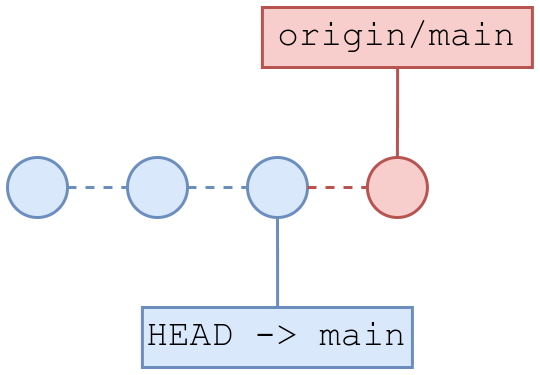
\includegraphics[width=0.5\linewidth]{fetch.png}
        \captionof{figure}{Estado de los commits tras el “fetch”}
    \end{center}


    \item \commandbox{git pull}

    En este caso se obtienen los commits del repositorio \textbf{y se aplican sobre la rama de trabajo actual}. Si tenemos cambios realizados en local, los cambios que obtenemos del repositorio \textbf{pueden entrar en conflicto con lo que tenemos}. Más adelante hablaremos de ello.

    De no existir conflictos, los cambios se aplican y el estado quedaría en ambos repositorios en el mismo punto exacto:

    \begin{center}
        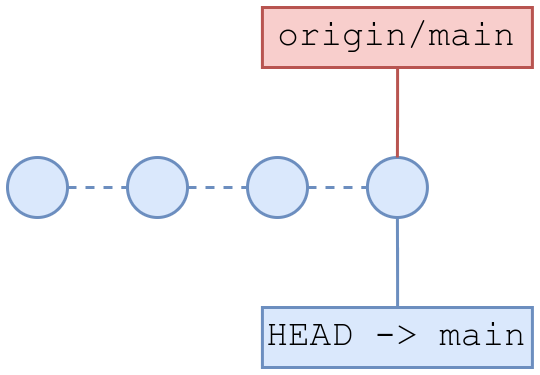
\includegraphics[width=0.5\linewidth]{pull.png}
        \captionof{figure}{Estado de los commits tras el “pull”}
    \end{center}
\end{itemize}

